\chapter{Introducci\'on}\label{capit:cap1}
\vspace{-2.0325ex}%
\noindent
\rule{\textwidth}{0.5pt}
\vspace{-5.5ex}% 
\newcommand{\pushline}{\Indp}% Indent puede ir o no :p

La interacción entre humanos se lleva a cabo gracias a la comunicación  que existe entre ellos, esta puede ser oral o escrita y generalmente viene acompañada de gestos realizados con la cara, manos o otra cualquier parte del cuerpo. 
Estos gestos sirven como complemento de la comunicación pues ayudan a que el mensaje sea percibido de manera correcta.

El creciente desarrollo de la tecnología en especial el desarrollo de computadoras, su incremento en procesamiento, la reducción de su tamaño y costo ha hecho que estas se incorporen cada vez más y sean parte esencial en nuestra vida diaria. De manera que se han creado y con ello estudiado distintas áreas de las ciencias computacionales, particularmente el área de interacción humano computadora (HCI, por sus siglas en ingl\'es Human Computer Interaction), el área encargada del estudio y diseño de la forma en que el humano interactua con la computadora. 
Uno de los objetivos principales de esta área es que la interacción se lleve acabo de manera natural. 
La manera en que el humano interactua con la computadora ha sido básicamente la misma desde que se empezó a tener acceso a ellas, fue hasta principios de esta década cuando la interacción ha empezado a cambiar pues ahora existen pantallas táctiles, reconocimiento de voz. Estas formas de interacción han sido aceptadas por los usuarios ya que hacen que la forma en que nos ``comunicamos'' con la computadora sea fácil y sencilla. No resulta extraño que los investigadores de HCI se hayan interesado en los gestos corporales, en especial los gestos realizados con las manos, para crear un ambiente natural entre el usuario y la computadora.  
Por lo que es necesario que la computadora pueda identificar la o las manos del usuario y reconocer el gesto que este realiza. 

A finales de los años noventa se empezaron a desarrollar t\'ecnicas para  el reconocimiento de gestos con las manos. Los primeros enfoques utilizaban como medio de captura sensores como guantes de datos, marcadores de colores y acelerómetros, los cuales se colocaban en la o las manos para poder capturar la posición e identificar la pose realizada. 
Las técnicas desarrolladas posteriormente obtienen la información necesaria para reconocer el gesto usando distintos tipos de imágenes o videos, que son obtenidos mediante diversos tipos de cámaras, por lo que no es necesario portar algún dispositivo para reconocer un gesto hecho con las manos.

Los métodos que utilizan imágenes o video son los más utilizados para realizar el reconocimiento de los gestos ya que la interacción entre el usuario y la computadora es más natural, el inconveniente con estos métodos es que es un problema difícil de resolver pues existen diversos aspectos que hay que tener en cuenta para obtener una buena precisión en el reconocimiento del gesto; por ejemplo tener en cuenta la resolución del dispositivo de captura, el ruido que existe en las imágenes, el tiempo de computo para realizar el procesamiento de las imágenes y las situaciones que se pueden presentar en la vida diaria que puedan entorpecer el reconocimiento del gesto. 

Aunque existe una gran variedad de métodos y sistemas que hacen el reconocimiento de gestos de las manos no existe alguno que presente en el reconocimiento un alto grado de precisión en todas las situaciones que se presentan en el mundo real, tales como; condiciones diversas de iluminación ya sea baja o alta, que funcionen en tiempo real, que funcionen a diversas escalas, es decir no importando el tamaño de la mano, que sea invariante a rotación, invariante al color de la piel y cuando exista alguna obstrucción parcial en el área de la mano.
Es por eso que se propone crear un sistema que reconozca gestos realizados con las manos, en situaciones que presentan baja iluminación y cuando existe obstrucción de los dedos. 
El sistema se enfoca en atacar estos problemas cuando las manos no se encuentran en movimiento, pero también se abordar\'an los gestos con las manos que involucran movimiento. El objetivo del sistema es mostrar que en ciertas ocasiones es posible obtener mayor precisión en el reconocimiento de los gestos utilizando como medio de captura dos sensores Kinect.   


%::::::::::::::::::::::::::::::::::::::::::::::::::::::::::::::::::::::::::::::::::::::::::::::::::::::::::::::::::::::::::::::::::


\section{Definici\'on del problema}\label{sec:DefinicionProblema}

Existen diversas técnicas que logran obtener buena precisión en el reconocimiento de gestos realizados con las manos. Sin embargo no hay técnicas que tengan buena precisión y que al mismo tiempo se adecuen a todo tipo de situaciones que se presentan en la vida real como: amigable con el usuario, invariante a la iluminación, rotación, el fondo, que funcione en tiempo real o cuando exista obstrucción en alguna parte de la mano o en los dedos.


%:::::::::::::::::::::::::::::::::::::::::::::::::::::::::::::::::::::::::::::::::::::::::::::::::::::::::::::::::::::::::::

\section{Justificaci\'on}\label{sec:Just}

Los métodos de reconocimiento de gestos desarrollados logran obtener un buen grado de reconocimiento en ciertas situaciones, generalmente en situaciones controladas.
De manera que se necesitan nuevos métodos que funcionen no solamente en condiciones ideales sino en situaciones que se presentan en la vida diaria y al mismo tiempo se obtenga un alto grado de precisión.  

Una vez logrado lo anterior se pueden desarrollar nuevas aplicaciones y tecnologías que ayuden a interactuar con naturalidad al usuario y la computadora.


%:::::::::::::::::::::::::::::::::::::::::::::::::::::::::::::::::::::::::::::::::::::::::::::::::::::::::::::::::::::::::::::::


\section{Objetivo general}\label{sec:ObjetivoGeneral}
 
Desarrollar un sistema de reconocimiento de gestos con las manos, gestos estáticos y dinámicos. El sistema debe funcionar bajo ciertas situaciones que se presentan en un ambiente natural. Es decir el sistema debe funcionar en circunstancias de baja iluminación y cuando exista obstrucción causada por los dedos en gestos dinámicos.


%:::::::::::::::::::::::::::::::::::::::::::::::::::::::::::::::::::::::::::::::::::::::::::::::::::::::::::::::::::::::::::::::


\section{Objetivos espec\'ificos}\label{sec:objetivosEspecificos}

\begin{itemize}
	\item Identificar los m\'etodos actuales de reconocimiento de gestos, estáticos y din\'amicos cuando existe baja iluminación  y cuando existe oclusión. 
	
	\item  Obtener conocimiento acerca del funcionamiento de sensor Microsoft Kinect.
	
	\item Desarrollar un sistema de reconocimiento de gestos estáticos y dinámicos, fusionando la información de los sensores de  profundidad de dos dispositivos kinect. El sistema desarrollado deberá funcionar en circunstancias de baja iluminación y también cuando existe oclusión, causada por los dedos. 
	
	\item Validar el sistema dise\~nado, en cuanto a su eficiencia con base al reconocimiento de los gestos, en circunstancias de baja iluminación y obstrucción. En el análisis del sistema se usar\'a información real.  
	
	\item Comparar y validar el modelo propuesto haciendo uso de uno y dos dispositivos Kinect. 
\end{itemize}


%::::::::::::::::::::::::::::::::::::::::::::::::::::::::::::::::::::::::::::::::::::::::::::::::::::::::::::::::::::::::::::::::::


\section{Limitaciones y suposiciones}\label{sec:Limitaciones&Suposiciones}

Gran porcentaje de los trabajos previos en el \'area de reconocimiento de gestos con las manos basados en el modelo de la visión  utilizan c\'amaras digitales o c\'amaras web. Esta investigación utiliza dos dispositivos Kinect, para obtener la información de entrada del sistema.

De  manera que las limitaciones del sistema propuesto están dadas por las características de dicho dispositivo, tales como la distancia  a la que se encuentran los dispositivos con el usuario y la resolución del sensor. 

Otra limitante es el número de gestos que podrá reconocer el sistema.


%::::::::::::::::::::::::::::::::::::::::::::::::::::::::::::::::::::::::::::::::::::::::::::::::::::::::::::::::::::::::::::::::::


\section{Reconocimiento de gestos con la manos}\label{sec:ReconocimientoGestos} 

Los gestos están definidos como movimientos del cuerpo expresivos y significativos que involucran a los  brazos, cabeza, cara, cuerpo, manos y dedos con la intención de transmitir información relevante o de interactuar con el ambiente \citep{Mitra2007}.

Los primeros enfoques para llevar acabo el reconocimiento de gestos con las manos fue usando modelos de contacto \citep{Rautaray2012} y \citep{Nayakwadi2014}.\\
El modelo utiliza dispositivos que est\'an en contacto f\'isico con la mano del usuario, ver la Figura \ref{fig:Modelos:1} para reconocer el gesto. Por ejemplo usan guantes de datos, marcadores de colores, acelerómetros y pantallas multi-toque. Este enfoque no es  tan aceptado pues entorpecen la naturalidad entre la interacción del humano y la computadora.\\
Los modelos basados en la visión, ver la Figura \ref{fig:Modelos:2} surgieron como respuesta a esta desventaja. Estos utilizan cámaras para extraer la información necesaria para realizar el reconocimiento. Los dispositivos van desde cámaras web hasta algunas más sofisticadas por ejemplo c\'amaras de profundidad.   

\begin{figure}[h!]
\begin{center}
\subfigure [Dispositivos basados en contacto: a la izquierda de la imagen se observan los guantes de datos \protect\footnotemark{}, en el centro los guantes de colores  \protect\footnotemark{}  y a la derecha se encuentra el dispositivo wii \protect\footnotemark{}.   \protect\addtocounter{footnote}{-3}]
{
    {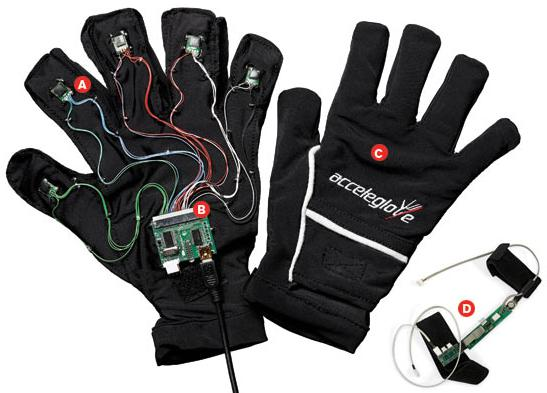
\includegraphics[scale=.25]{./Figures/Dataglove.jpg}}  \qquad
	{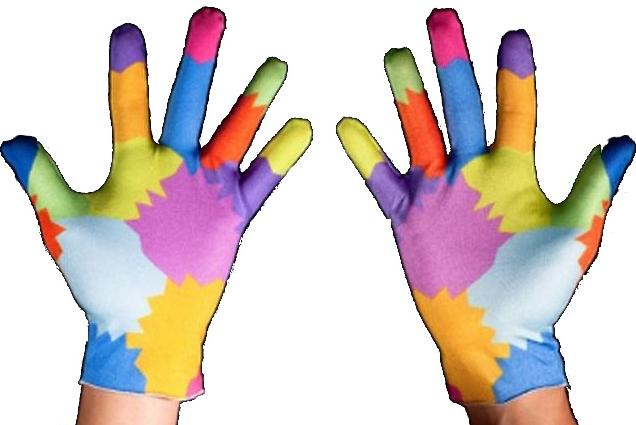
\includegraphics[scale=.25]{./Figures/colorGloves.jpg}} \qquad   	
	{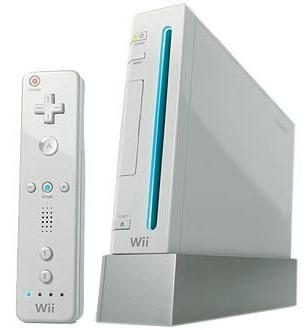
\includegraphics[scale=.29]{./Figures/wii.jpg}} 	  	
	\label{fig:Modelos:1}
}
\subfigure [Dispositivos basados en visión: en la imagen se observan distintos tipos de cámaras. A la izquierda de la imagen se observa una cámara web \protect\footnotemark{}, en el centro una cámara digital \protect\footnotemark{} y a la derecha de la imagen una cámara  TOF \protect\footnotemark{}.]
{
	{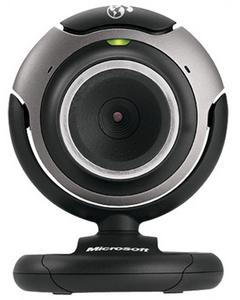
\includegraphics[scale=.3]{./Figures/webcam.jpg}} 		\qquad
	{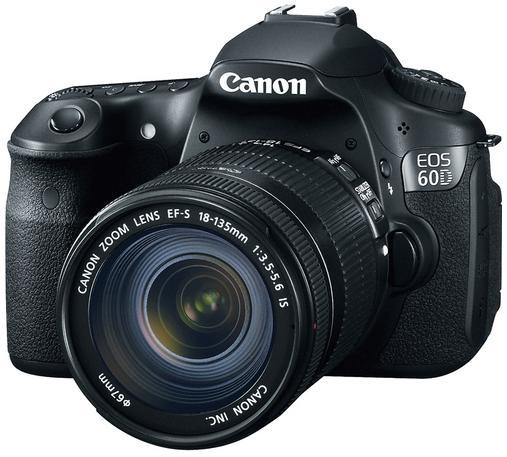
\includegraphics[scale=.2]{./Figures/digitalCamera.jpg}}  \qquad
	{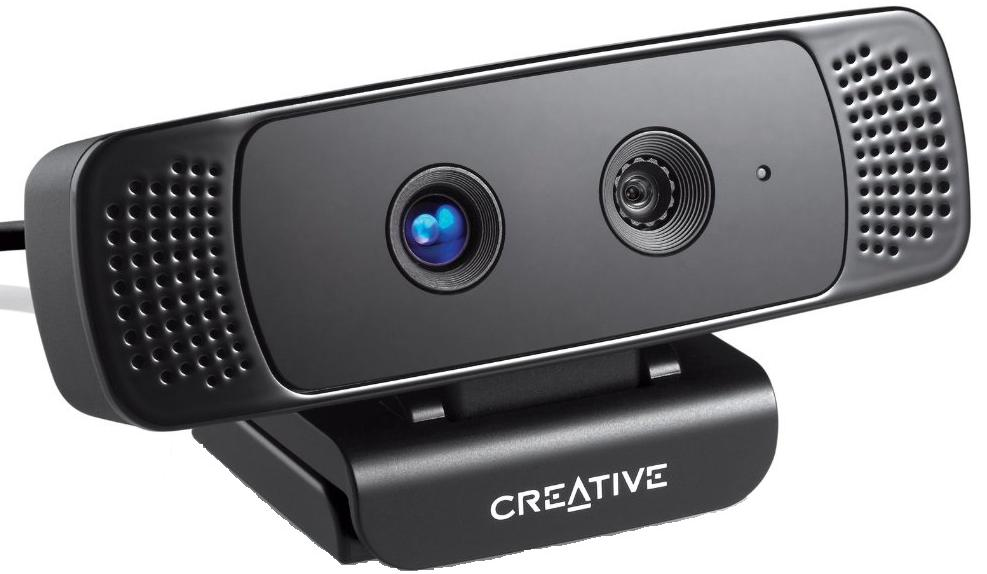
\includegraphics[scale=.15]{./Figures/TOF.jpg}} 
    \label{fig:Modelos:2} 
}
\caption{Dispositivos utilizados para la captura de gestos.} 
\label{fig:Modelos} 
\end{center}
\end{figure} 

En este trabajo, se toma el enfoque basado en la visión debido a que se busca obtener un sistema que para el usuario la interacción sea natural y la manera de lograrlo es tomando este enfoque.  

\footnotetext[1] {\url{ http://www.technologyreview.com/article/414021/open-source-data-glove/}} \stepcounter{footnote}
\footnotetext[2] {\url{http://www.digitaltrends.com/computing/the-gloves-that-could-change-the-world/}}
\footnotetext[3] {\url{https://www.nintendo.es/Wii/Wii-94559.html}}

\footnotetext[4] {\url{http://es.ccm.net/download/descargar-2562-driver-de-microsoft-lifecam-vx-3000}}
\footnotetext[5] {\url{http://www.canon.com.mx/ficha.aspx?id=722}} 
\footnotetext[6] {\url{http://us.creative.com/p/web-cameras/creative-senz3d}}


%::::::::::::::::::::::::::::::::::::::::::::::::::::::::::::::::::::::::::::::::::::::::::::::::::::::::::::::::::::::::::::::::::


\section{Estado del arte}\label{sec:EstadoDelArte} 

En esta sección se presentan los trabajos relevantes de cada uno de estos enfoques y también se mencionan algunos de los sistemas comerciales importantes. 

\subsection{Modelos de contacto}
 
Los primeros trabajos de reconocimiento de gestos con las manos utilizan este modelo, actualmente se sigue utilizando pero en menor grado. 

Un método de reconocimiento de gestos con las manos que utiliza guantes de datos \citep{Yoon2012} propone un sistema de reconocimiento de gestos estáticos, el cual reconoce veinticuatro gestos tomados del Lenguaje de Señas Americano, ASL (por sus siglas en inglés, American Sign Lenguaje). Este modelo consta de tres etapas. 
La primera etapa del sistema consiste en capturar la información proporcionada por un guante de datos, la cual esta siendo enviada por un protocolo de control de transmisión TCP, (por sus siglas en inglés, Transmission Control Protocol).
Una vez que la información es recibida, los datos son pre-procesados, es decir son normalizados y las características son extraídas, las características son las correlaciones que existe entre los ejes.   
La clasificación de gesto se realiza con un modelo de mezclas adaptativo. Para entrenar el modelo de mezclas se toman datos de cinco personas, trescientas muestras de cada gestos, ocho mil por cada participante. Se realizaron pruebas con estos mismos datos; con un sujeto se alcanzó una precisión de $93.38 \%$ con los demás participantes se obtuvo una precisión de $89.97 \%$.  
La principal desventaja del sistema es que este requiere tiempo para adaptarse a distintos usuarios. Otra desventaja para este sistema es que solo reconoce gestos estáticos. 

A finales del año 2014 se lanzó el dispositivo MYO \footnote{\url{https://www.thalmic.com/en/myo/}}, el cual reconoce gestos dinámicos, se muestra en la Figura \ref{fig:Myo}. Este aparato es un brazalete que reconoce cinco gestos dinámicos. Leyendo la actividad de los músculos del antebrazo y mandando estas señales vía bluetooth a la computadora donde estas señales son procesadas. \footnote{\url{http://www.digitaltrends.com/pc-accessory-reviews/myo-gesture-control-armband-review/}} 

No se cuenta con la informacion detallada del funcionamiento de MYO, lo único que se conoce es que el reconocimiento consta de tres etapas \footnote{\url{https://www.quora.com/How-does-MYO-wearable-gesture-control-work}}. La primera es la adquisición de la señales eléctricas que producen los músculos esqueléticos del antebrazo, las cuales son capturadas mediante sensores que detectan la actividad eléctrica, giroscopio, acelerómetro y magnetómetro; en la segunda etapa se amplifica la señal y se aplica un filtro pasa banda. Por último se realiza el procesamiento de la señal donde se reconoce el gesto usando un algoritmo de aprendizaje de máquina desarrollado por la compañía.  

\begin{figure}[h!]
\begin{center}
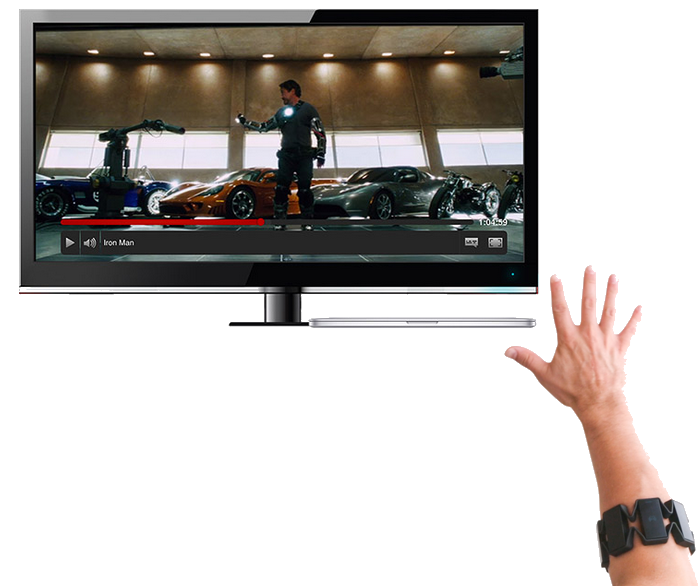
\includegraphics[scale=.5]{./Figures/MYO.png}
\end{center}
\caption{Ejemplo del reconocimiento del gesto usando MYO, controlando el volumen de la computadora. El dispositivo es el que aparece en el brazo del sujeto. Imagen recuperada de \protect\footnotemark{}.}
\label{fig:Myo}
\end{figure}

\footnotetext{\url{https://www.myo.com/}} 

MYO funciona en cualquier ambiente donde haya variaciones en la iluminación y es invariante a rotación.
La principal desventaja es la calibración debido a que puede ser tediosa pues es necesario realizar un considerable número de repeticiones de algunos gestos. Otra desventaja es que tiene una cantidad considerable de falsos positivos \footnote{ \url{http://myogroupfive.blogspot.mx/2013/11/benefits-disadvantages-for-business\_ 24.html}}. Un punto importante es que para el uso del dispositivo es preferible el uso de manga corta. 


\subsection{Modelos basados en la visión}   

Este modelo es el más popular debido a la variedad de sus aplicaciones y la diversidad de cámaras existentes que proporcionan distinto tipo de información. Existe una gran gama de datos que se pueden extraer con este modelo, usando las técnicas o métodos adecuados para el tipo de datos extraído se puede llegar a tener gran precisi\'on en el reconocimiento. Enseguida se presenta tres trabajos relevantes los cuales utilizaron distintos tipos de cámaras y número de ellas. 

%En el trabajo propuesto por \cite{Premaratne2013} realizan un modelo de reconocimiento de gestos estático y dinámico basados en el algoritmo de Lucas-Kanade. Las principales ventajas de este método son que es invariante a rotación, escala y al fondo. Aunque el modelo es afectado por los cambios en la iluminación.
%::::::::::::::::::::::::::::::::::::::::::::::::::::::::::::::::::::::::::::::::::::::::::::::::::::::::

En trabajo de \citep{Huang2011} se propone un método que reconoce once gestos estáticos y dinámicos. El sistema propuesto utiliza una cámara CCD para obtener la información de entrada. La aportación del trabajo es la segmentación de la mano que se lleva acabo usando filtros de Gabor. El sistema es robusto a la iluminación. 
 
Antes de realizar la segmentación de la mano se le aplica a la imagen un preprocesamiento que consiste en aplicar un filtro de Gabor. Después se escoge uno de los tres modelos del color; YCbCr, Gaussiano o Soriano, tomando en cuenta un nivel de gris.  
Una vez que es realizado el preprocesamiento el paso siguiente es segmentar de la imagen de la mano el antebrazo, para esto se hace un barrido de la imagen por filas. Se segmenta la mano tomando en cuenta la distancia que existe entre la parte superior de la imagen y el número máximo de pixeles de un solo valor (el valor mayor del histograma).

Una vez realizada la segmentación se obtienen las características necesarias para el reconocimiento. Las características son obtenidas utilizando análisis de componentes principales, PCA (por sus siglas en inglés, Principal Component Analysis).

La clasificación se realiza por medio de máquinas de vectores de soporte, SVM (por sus siglas en inglés, Support Vector Machines).   

La precisión del reconocimiento varía dependiendo de las imágenes, si son reales o si se les aplica antes un filtro de Gabor. También cambia si el usuario usa manga corta o larga.  
Las principales ventajas son que el sistema funciona con cambios en la iluminación y es robusto a la rotación y escala. Una limitación de sistema es que no es tratado el problema de obstrucción. 

%:::::::::::::::::::::::::::::::::::::::::::::::::::::::::::::::::::::::::::::::::::::::::::

Otro trabajo propuesto \citep{Caputo2012} realiza el reconocimiento de  gestos dinámicos y estáticos, estos últimos son utilizados para determinar el inicio y el término de los gestos dinámicos. Se utilizan dos sensores Kinect y una cámara web Logitech C910 de alta definición para capturar los gestos. El trabajo está compuesto de cuatro etapas.

La primera es la configuración de los dispositivos de captura de datos del sistema. Los dos sensores Kinect son calibrados entre ellos para generar un sistema de coordenadas que está basado en la ubicación de la  manos y la cabeza. La cámara y los dispositivos Kinect no son sincronizados entre sí.  

La parte de la detección y seguimiento  se lleva acabo utilizando la librería OPENNI, en específico usando la detección del esqueleto. El esqueleto nos proporciona el punto de la palma de la mano por la cual la región de interés, ROI (por sus siglas en inglés, Region of Interest) es seleccionada. Para tener una  mejor aproximación de la localización de la mano, se utiliza la cámara RGB. La localización de la mano se realiza convirtiendo la imagen en una imagen binaria, usando un umbral que es determinado por el espacio del color HSV (Matiz, Saturación, Valor); son utilizados guantes neón color rosa o verde para ubicar con mayor facilidad las manos.   

Una vez obtenida la imagen binaria se calcula el contorno de la mano usando el algoritmo de \citep{Chang2004}, dicho contorno es extraído como polígono y  es simplificado con el algoritmo de Douglas Peuker. 

El reconocimiento del gesto utiliza el empatamiento de polígonos, el cual se basa en comparar dos polígonos, mediante distancias. Esto usando distancia de momentos HU y ángulo de giro. 
Los gestos 3D son calculados usando la diferencia de las posiciones de la mano en cada cuadro. Las fórmulas para calcular estos gestos depende de qué gesto se  realice.  
Para probar la precisión del sistema se crearon dos bases de datos: una con $120$ polígonos etiquetados que representan once gestos y otra con $144$ gestos de tres personas distintas realizando los once gestos. La precisión obtenida usando la distancia de ángulo de giro es de $85 \%$, usando la distancia de momentos HU la precisión es de $58 \%$.  

%::::::::::::::::::::::::::::::::::::::::::::::::::::::::::::::::::::::::::::::::::::::::::::::::::::::::

Otra aportación importante fue hecha por \citep{Kang2013} ellos proponen un sistema de reconocimiento de  gestos estáticos utilizando el sensor Kinect como dispositivo de captura de los gestos. El sistema reconoce veinticuatro gestos, los cuales pertenecen al ASL, el reconocimiento es realizado en cuatro etapas, las cuales se explican a continuación.  

En la primera etapa la imagen es capturada y la mano junto con el antebrazo son segmentados del fondo. Las imágenes de entrada del sistema son proporcionadas por el sensor de profundidad del Kinect, la mano es detectada usando el SDK (Software Developmet Kit) del Kinect, que proporciona el punto de la palma de la mano, la región de interés es seleccionada usando este punto, donde  solo se encuentra la mano y parte del antebrazo.   

Después se extraen las características, las cuales son extraídas usando Histogramas Orientados a Gradientes, HOG (Histogram of Oriented Gredient).  

Para la clasificación de los gestos, se utiliza el algoritmo de aprendizaje de máquina, máquinas de soporte vectorial.
Para el entrenamiento se utilizaron $2400$ imágenes, cien por cada letra del alfabeto. Se encontró que existen gestos ambiguos, es decir que no se pueden clasificar correctamente, estos son los gestos que representan la letras A, E, M, N, S, T. 
Se realizó una prueba en linea, donde los gestos aparecían aleatoriamente para ser clasificados. La precisión de todos los gestos se encuentra alrededor de $92.8 \%$, pero el de los gestos ambiguos es $72.9 \%$
Por último una interfaz gráfica es mostrada donde se aprecia el reconocimiento de los gestos en tiempo real.  

%::::::::::::::::::::::::::::::::::::::::::::::::::::::::::::::::::::::::::::::::::::::::::::::

%La SECCIÓN A pesar que la mayoría de los modelos vistos en la parte de arriba solucionan muchos de los problemas de los modelos basados en la visi\'on. Ninguno de ellos puede resolver el problema de iluminaci\'on y oclusi\'on, formada por lo dedos. All\'i la importancia de la investigaci\'on propuesta, pues dar\'a soluci\'on a estos inconvenientes al momento de reconocer los gestos.
 
\subsection{Sistemas comerciales}

Existen dispositivos como: Leap Motion \footnote{\label{LeapMotionFN} \url{https://www.leapmotion.com/}}, MYO \footnote{\label{MyoFN}  \url{https://www.myo.com/}} y software como Flutter \footnote{\label{FlutterFN} \url{ https://flutterapp.com/}}, que realizan el reconocimiento de gestos, este reconocimiento es aplicado para controlar la computadora. Algunos de estos dispositivos comerciales tienen  buen rendimiento en cuanto a la precisión y a sobrellevar los problemas del reconocimiento de gestos. El inconveniente es que los desarrolladores de los dispositivos o software no dan a conocer los detalles de cómo solucionan algunos de los problemas o cómo mejoran la precisión. 
Enseguida se describen los sistemas mencionados anteriormente.
 
El dispositivo Leap Motion (Figura \ref{fig:LeapMotion}) fue creado para el seguimiento de manos y dedos. Este también hace el reconocimiento de ciertos gestos estáticos y dinámicos. El dispositivo consta de tres emisores y dos cámaras infrarrojas, estos sensores capturan los datos crudos en un rango de $60 \times 60 \times 60$ $cm.$ y con la información capturada se construye un modelo 3D de las manos \citep{Weichert2013}. 

\begin{figure}[h!]
\begin{center}
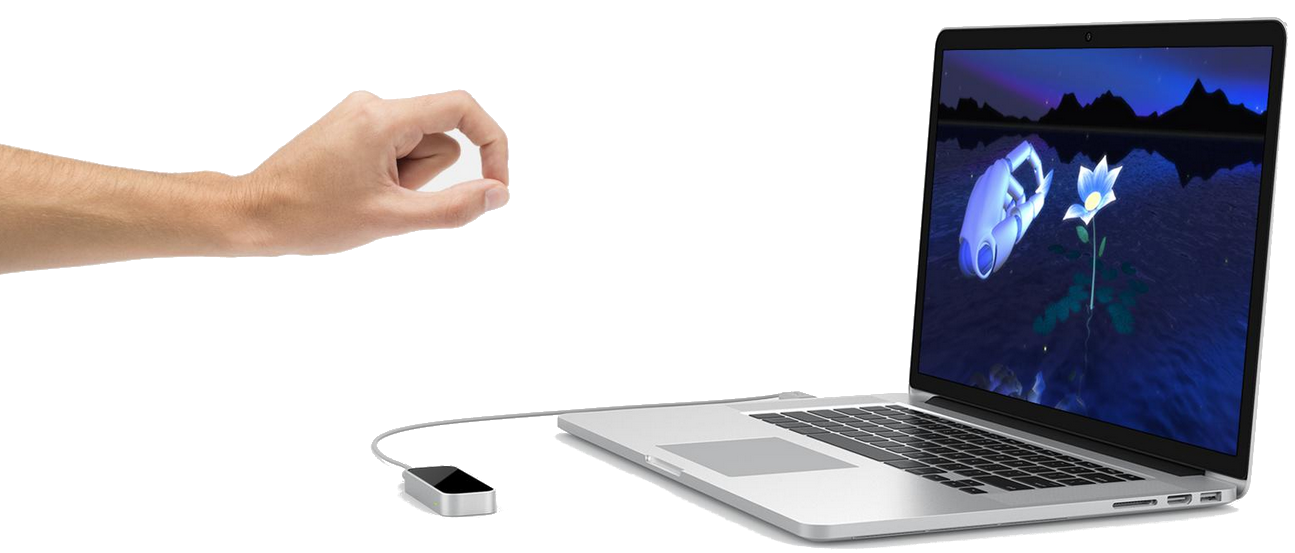
\includegraphics[scale=.3]{./Figures/LeapMotion.png}
\end{center}
\caption{Ejemplo del reconocimiento del gesto usando Leap Motion, mostrando una aplicación donde los gestos son representados en 3D. Leap Motion es el dispositivo que se encuentra conectado a la laptop. Imagen recuperada de \textsuperscript{\ref{LeapMotionFN}}.}
\label{fig:LeapMotion}
\end{figure}

El proceso de captura de los datos, la segmentación, la extracción de características, el seguimiento y el reconocimiento del dispositivo no se conoce a detalle, pues no ha sido publicado.
Solo se conoce \footnote{\url{http://goo.gl/INzrdR}} que se utilizan tres cámaras infrarrojas. Con la imágenes obtenidas con se hace una representación 3D de las manos. Antes de realizar el modelo,  se sustrae el fondo de las imágenes para eliminar el ruido generado por la iluminación u otros objetos. 
Para realizar el seguimiento se extraen la características. Una de ellas son los dedos, el algoritmo de seguimiento interpreta la información 3D e infiere la posición de los objetos ocluidos. Se aplican filtros para suavizar los datos. 

Enseguida se explica el software de reconocimiento de gestos estáticos Flutter, ver la Figura \ref{fig:Flutter}, el cual reconoce cuatro gestos estáticos usando la cámara web como dispositivo de entrada. 

Se desconoce cómo funciona el software, solo se sabe que la mano es detectada por la cámara, para que la detección sea correcta la mano tiene que estar totalmente frente a la cámara web. Los algoritmos utilizados para el reconocimiento no se conocen.  
\begin{figure}[h!]
\begin{center}
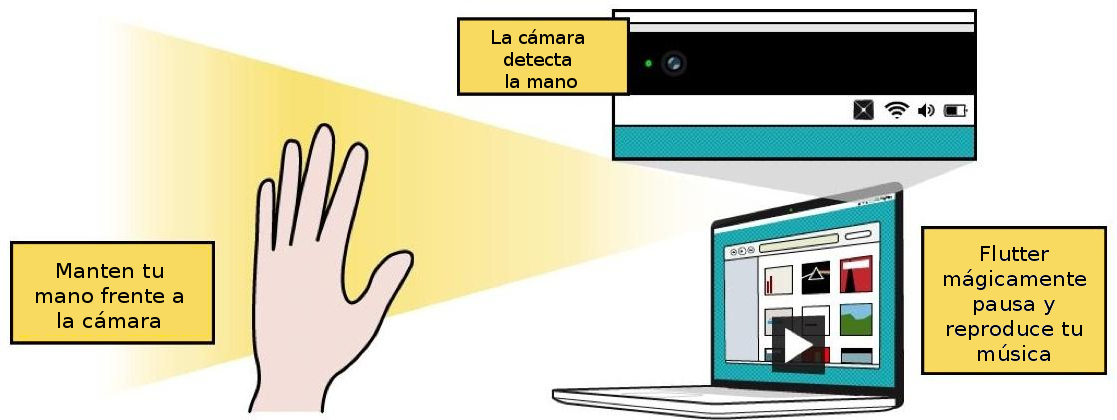
\includegraphics[scale=.4]{./Figures/Flutter.jpg}
\end{center}
\caption{La imagen anterior representa el funcionamiento del software Flutter. Imagen recuperada de \textsuperscript{\ref{FlutterFN}}.}
\label{fig:Flutter}
\end{figure}

Flutter permite controlar aplicaciones multimedia como: YouTube \footnote{\url{https://www.youtube.com/}} ,VLC \footnote{\url{http://www.videolan.org/vlc/}}, Spotify \footnote{\url{https://www.spotify.com/}}, Netflix \footnote{\url{https://www.netflix.com/}}. Las limitaciones del software son que solo reconoce gestos estáticos. Una desventaja es que presenta falsos positivos al reconocer acciones del usuario.  

%::::::::::::::::::::::::::::::::::::::::::::::::::::::::::::::::::::::::::::::::::::::::::::::::::::::::: 

Aunque estos dispositivos y software para reconocer gestos solucionan algunos problemas importantes en el área, sigue existiendo el problema de bloqueo e iluminación.
De allí la importancia que existan nuevos modelos que ataquen estos problemas que se presentan frecuentemente en el reconocimiento de los gestos.
  
\section{Organizaci\'on de la tesis}\label{OrganizacionTesis}

La tesis se encuentra distribuida de la siguiente manera: la segunda sección presenta los fundamentos teóricos como base para la comprensión del tema. La tercera sección presenta la metodología utilizada en el sistema propuesto. En la cuarta sección se encuentran los detalles de la implementación del sistema. En la quinta sección están las pruebas realizadas al sistema junto con los resultados y las discusiones de estos. Finalmente la sexta sección presenta las conclusiones generales del sistema y el trabajo a futuro. 

